\section{Result 2: VC and Rademacher bounds for the linear filter}
\label{sec:result-2}

Feature vectors $x\in\R^{k+1}$ ($k$ features and the intercept coordinate), $\norm{x}\le C=1$;
classifiers $x\mapsto\operatorname{sign}(w\cdot x)$; $L_{01}(w)=\P_Q(y\,w\cdot x\le0)$. The
logistic loss of the margin $u=y\,w\cdot x$ is $\ell(u)=\ln(1+e^{-u})$, and
$\psi(u)=\min(\ell(u),\ln2)$ is its clipped version; $\hat L$ denotes training averages. Training
always minimizes the logistic loss; $\psi$ is used only to evaluate the bound.

\begin{theorem}[Result 2]
\label{thm:2}
Let $S$ be $n$ i.i.d.\ examples from $Q$.
\begin{enumerate}[label=(\roman*)]
  \item (VC.) If $n\ge k+1$, with probability at least $1-\delta$, for every $w\in\R^{k+1}$,
  \[ L_{01}(w)\le\hat L_{01}(w)+\sqrt{\frac{8\bigl((k+1)\ln\frac{2en}{k+1}+\ln\frac4\delta\bigr)}{n}}. \]
  \item (Rademacher, clipped loss.) With probability at least $1-\delta$, for every $w$ with
  $\norm{w}\le B$,
  \[ L_{01}(w)\le\frac1{\ln2}\Bigl(\hat L_{\psi}(w)+\frac{2B}{n}\sqrt{\textstyle\sum_{i}\norm{x_i}^2}
     +3\ln2\,\sqrt{\frac{\ln(2/\delta)}{2n}}\Bigr). \]
  Applying (ii) at $\delta/G$ to each of $G$ grid values of $B$ makes all $G$ hold at once (union
  bound), so $B$ may be chosen after seeing the data.
\end{enumerate}
\end{theorem}

\begin{proof}
(i) Linear classifiers with an intercept on $\R^k$ have VC dimension $k+1$: the origin and the
$k$ unit vectors are shattered, and by Radon's theorem any $k+2$ points split into two sets whose
convex hulls intersect, so they cannot be separated. Our classifiers on $x=(z,1)$ are exactly
this class on $z\in\R^k$ (the convention at $w\cdot x=0$ does not change this). \Cref{lem:uc} with Sauer--Shelah, $\Pi(2n)\le(2en/d)^d$ for $d=k+1\le n$,
gives $\P(\sup_w\abs{L_{01}(w)-\hat L_{01}(w)}>\epsilon)\le4(2en/d)^de^{-n\epsilon^2/8}$. Setting
this to $\delta$ gives (i); the lemma's condition $n\epsilon^2\ge8\ln(4/\delta)\ge2$ holds.

(ii) Let $\cF=\{(x,y)\mapsto\psi(y\,w\cdot x):\norm{w}\le B\}$ and let
$\hat R_S(\cF)=\E_\sigma\sup_{f\in\cF}\frac1n\sum_i\sigma_if(z_i)$ be its empirical Rademacher
complexity, with independent fair signs $\sigma_i$.
\begin{enumerate}[label=(\alph*),leftmargin=*]
  \item \emph{Generalization bound.} If every $f\in\cF$ takes values in an interval of length
  $\Delta$, then with probability at least $1-\delta$, for all $f\in\cF$,
  $\E f\le\hat\E_Sf+2\hat R_S(\cF)+3\Delta\sqrt{\ln(2/\delta)/(2n)}$. Proof: changing one point
  changes $\Phi(S)=\sup_f(\E f-\hat\E_Sf)$ by at most $\Delta/n$, so McDiarmid's inequality \citep{mcdiarmid1989method} gives
  $\Phi(S)\le\E\Phi+\Delta\sqrt{\ln(2/\delta)/(2n)}$ with probability $1-\delta/2$. Symmetrization
  with a ghost sample and random signs (as in \cref{lem:uc}) gives $\E\Phi\le2\E\hat R_S(\cF)$.
  $\hat R_S(\cF)$ also changes by at most $\Delta/n$ per point, so McDiarmid again gives
  $\E\hat R_S\le\hat R_S+\Delta\sqrt{\ln(2/\delta)/(2n)}$ with probability $1-\delta/2$. A union
  bound over the two events gives the claim, which holds for all $f$ at once because it bounds
  the supremum.
  \item \emph{Range.} $\psi$ takes values in $(0,\ln2]$, so $\Delta\le\ln2$ for every $B$.
  \item \emph{Contraction.} $\abs{\ell'(u)}=1/(1+e^{u})\le1$, so $\ell$ is 1-Lipschitz, and so is
  $\psi$ ($\abs{\min(a,c)-\min(b,c)}\le\abs{a-b}$). By the contraction lemma of
  \citet[ch.~26]{shalevshwartz2014understanding} (if $\varphi_1,\dots,\varphi_n$ are $\rho$-Lipschitz,
  applying $\varphi_i$ to the $i$-th coordinate of every vector in a set $A\subset\R^n$ multiplies its
  Rademacher complexity by at most $\rho$; this version has no absolute values and needs no
  condition $\varphi_i(0)=0$), applied to the margin vectors $(y_i\,w\cdot x_i)_{i\le n}$ with
  $\varphi_i=\psi$, $\hat R_S(\cF)\le\hat R_S(\{(x,y)\mapsto y\,w\cdot x\})$.
  \item \emph{Margin class.} For fixed labels, $\sigma_iy_i$ are again independent fair signs, so
  the margin class has the same complexity as $\{x\mapsto w\cdot x:\norm w\le B\}$.
  \item \emph{Linear class.} By Cauchy--Schwarz, then Jensen, then $\E[\sigma_i\sigma_j]=\mathbb 1[i=j]$,
  \[ \E_\sigma\sup_{\norm w\le B}\frac1n\sum_i\sigma_i\,w\cdot x_i=\frac Bn\E_\sigma\Bigl\lVert\sum_i\sigma_ix_i\Bigr\rVert
     \le\frac Bn\Bigl(\E_\sigma\Bigl\lVert\sum_i\sigma_ix_i\Bigr\rVert^2\Bigr)^{1/2}=\frac Bn\sqrt{\textstyle\sum_i\norm{x_i}^2}. \]
  \item \emph{From $\psi$ to 0-1.} If $u\le0$ then $\ell(u)\ge\ell(0)=\ln2$, so $\psi(u)=\ln2$ and
  $\mathbb 1[u\le0]\le\psi(u)/\ln2$; hence $L_{01}(w)\le\E\psi/\ln2$.
\end{enumerate}
Combining (a)--(f) gives (ii). For the grid, each bound fails with probability at most $\delta/G$,
so all hold together with probability at least $1-\delta$, in particular for the chosen $B$.
\end{proof}

\begin{remark}[Unclipped version]
With $\ell$ in place of $\psi$ only step (b) changes: since $\abs{y\,w\cdot x}\le BC$ and
$\ln(1+e^{a})-\ln(1+e^{-a})=a$, $\ell$ ranges over an interval of length exactly $BC$, and the last
term becomes $3BC\sqrt{\ln(2/\delta)/(2n)}$, which grows with $B$. It is computed for comparison.
\end{remark}

\begin{inshort}
\begin{enumerate}[leftmargin=*]
  \item VC: half-spaces with intercept in $\R^k$ have $d=k+1$; plug into the uniform-convergence
    bound $4(2en/d)^de^{-n\epsilon^2/8}=\delta$. The gap is $\approx\sqrt{d\ln n/n}$: needs $n\gg d$.
  \item Rademacher: McDiarmid + symmetrization; clipped logistic loss has range $\le\ln2$ whatever
    $B$; contraction (1-Lipschitz); random signs absorb the labels; Cauchy--Schwarz + Jensen give
    $\frac Bn\sqrt{\sum\norm{x_i}^2}$; a mistake costs $\psi=\ln2$, so divide by $\ln2$.
    No dimension anywhere, only $B$ and the feature norms.
  \item A grid of $G$ values of $B$ costs $\ln G$ inside the square root.
\end{enumerate}
\end{inshort}

\paragraph{Measured vs.\ theory (E2a).} Overlapping regime; $\ETwoRepeats$ repeats on fresh dies,
$n=\ETwoNFirst,\dots,\ETwoNLast$. The projected-gradient fit runs at every $B\in\{2^{-1},\dots,2^8\}$
($G=10$) and $B$ is chosen by validation error; both bounds are evaluated for that filter. The
check fixed before running (both bounds above the test error in at least 95\% of runs) holds for
every feature set.

\begin{center}
\small
\resizebox{\linewidth}{!}{%
\begin{tabular}{lcccccccc}
\toprule
& & & \multicolumn{2}{c}{bound $\ge$ test error} & \multicolumn{2}{c}{first $n$ with bound $<\TrivialError$}
& \multicolumn{2}{c}{at $n=\ETwoNLast$} \\
\cmidrule(lr){4-5}\cmidrule(lr){6-7}\cmidrule(lr){8-9}
features & $k$ & $L(h^\star)$ & VC & Rad. & VC & Rad. & test error & VC / Rad.\ bound \\
\midrule
hand-crafted & 10 & $\ETwoHandLStar$ & \ETwoHandFracVC & \ETwoHandFracRad & $\ETwoHandFirstNVC$ & $\ETwoHandFirstNRad$ & $\ETwoHandTestLast$ & $\ETwoHandVCLast$ / $\ETwoHandRadLast$ \\
PCA-16 & 16 & $\ETwoPcaSixteenLStar$ & \ETwoPcaSixteenFracVC & \ETwoPcaSixteenFracRad & $\ETwoPcaSixteenFirstNVC$ & $\ETwoPcaSixteenFirstNRad$ & $\ETwoPcaSixteenTestLast$ & $\ETwoPcaSixteenVCLast$ / $\ETwoPcaSixteenRadLast$ \\
PCA-64 & 64 & $\ETwoPcaSixtyFourLStar$ & \ETwoPcaSixtyFourFracVC & \ETwoPcaSixtyFourFracRad & $\ETwoPcaSixtyFourFirstNVC$ & $\ETwoPcaSixtyFourFirstNRad$ & $\ETwoPcaSixtyFourTestLast$ & $\ETwoPcaSixtyFourVCLast$ / $\ETwoPcaSixtyFourRadLast$ \\
CNN-384 & 384 & $\ETwoCnnFullLStar$ & \ETwoCnnFullFracVC & \ETwoCnnFullFracRad & $\ETwoCnnFullFirstNVC$ & $\ETwoCnnFullFirstNRad$ & $\ETwoCnnFullTestLast$ & $\ETwoCnnFullVCLast$ / $\ETwoCnnFullRadLast$ \\
\bottomrule
\end{tabular}}
\end{center}

The VC bound beats the trivial error $\TrivialError$ only for the hand-crafted features (from
$n=\ETwoHandFirstNVC$); for CNN-384 it would need $n\approx\ETwoCnnFullVCNeedN$. The usual expectation
that the dimension-free bound is tighter fails: at the validated $B$ the Rademacher bound is
$\ETwoRadLastMin$--$\ETwoRadLastMax$, above VC for every feature set. Choosing $B$ to minimize the
Rademacher bound instead trades error for bound. For CNN-384 that filter's bound is tighter than VC
($\ETwoCnnFullRadCertLast$ vs $\ETwoCnnFullVCLast$), though neither is below the trivial $\TrivialError$,
and its test error is $\ETwoCnnFullRadCertTestLast$ instead of $\ETwoCnnFullTestLast$
(\cref{sec:looseness}).

\paragraph{Approximation vs.\ estimation (E2b).} $L(h^\star)$ is the test error of the logistic fit on
the population pool, an upper estimate of the best-in-class error. Richer CNN features lower it
and raise the estimation error at small $n$ (at $n=\ETwoNFirst$: $\ETwoPcaSixteenEstFirst$,
$\ETwoPcaSixtyFourEstFirst$, $\ETwoCnnFullEstFirst$ for PCA-16, PCA-64, CNN-384), so their curves
cross. The ten hand-crafted features match CNN-384's $L(h^\star)$ ($\ETwoHandLStar$ vs.\
$\ETwoCnnFullLStar$) with an estimation error of only $\ETwoHandEstFirst$ at $n=\ETwoNFirst$, and are
best at every $n$ tested.

\begin{figure}[tb]
  \centering
  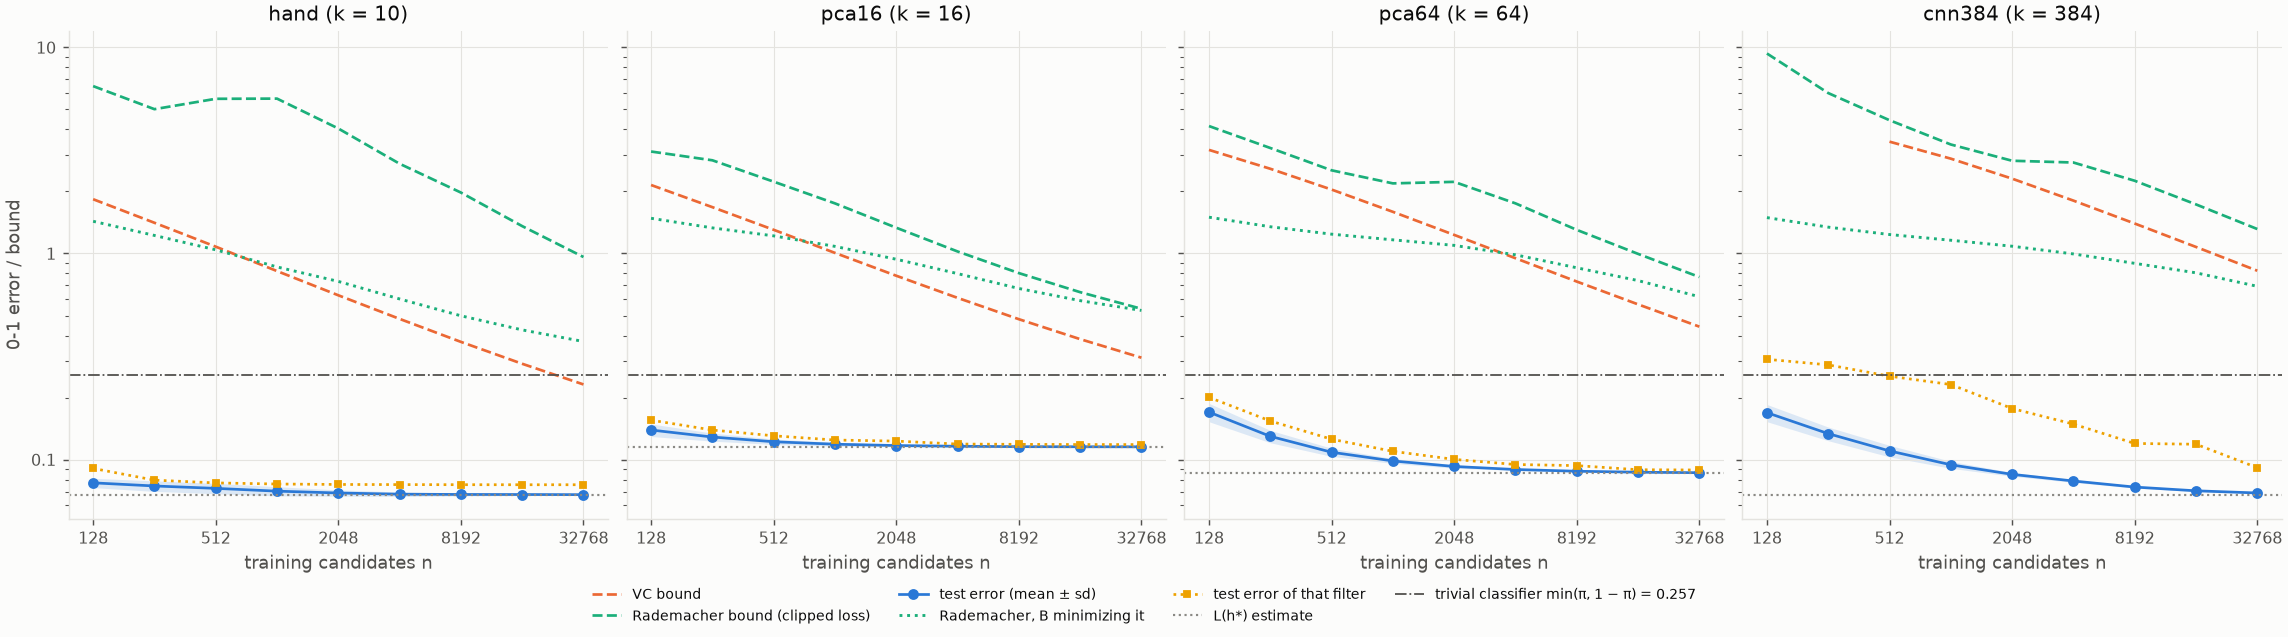
\includegraphics[width=0.8\linewidth]{../figures/e2a_bounds.png}\\[4pt]
  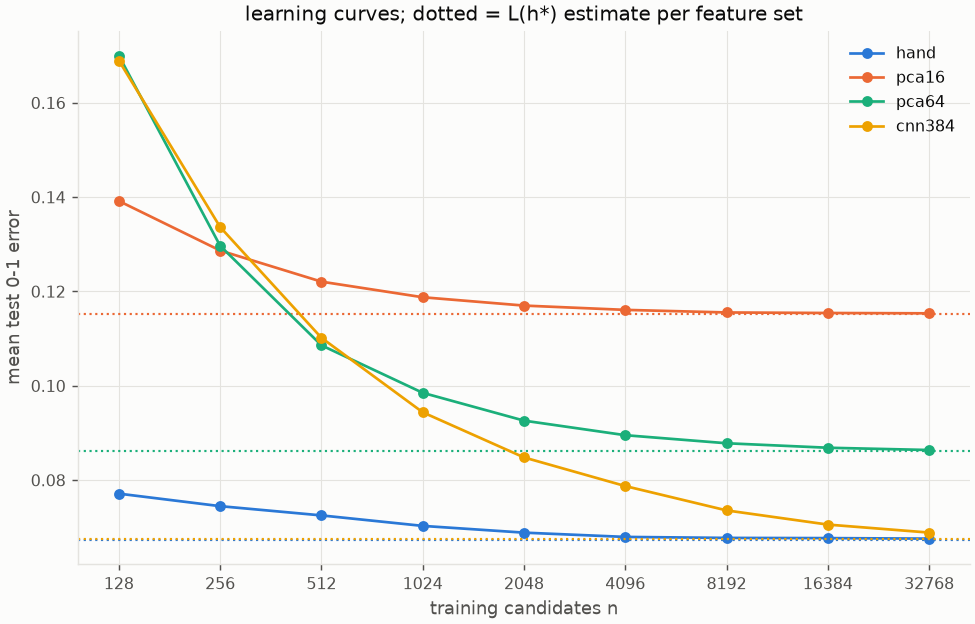
\includegraphics[width=0.5\linewidth]{../figures/e2b_curves.png}
  \caption{Top (E2a): test error and both Result~2 bounds per feature set; dash-dotted: the
  trivial error $\min(\pi,1-\pi)$. Bottom (E2b): learning curves with the $L(h^\star)$ estimates
  (dotted).}
  \label{fig:e2}
\end{figure}
